\section{EpToTester}
\label{sec:epto}
\sys is a framework using Docker and Docker Swarm. It is designed to ease the deployment of large scale distributed systems and in this particular case \jgroups and \epto. We use \sys to assess the claims made in \autocite{matos2015epto}. Although the implementation of \epto is written with benchmarking in mind, the code can be adapted for real applications with only minimal changes to the sources. We  use \sys instead of other solutions such as SPlay, which only supports LUA, as we need to test existing protocols written in different programming languages.
\subsection{Deployment}
\begin{figure}[htp]
	\centering
	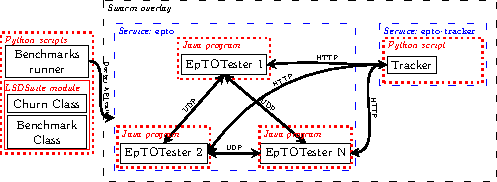
\includegraphics[width=\linewidth]{figures/complete-architecture.pdf}
	\vspace{-2mm} 
	\caption[Caption]{\epto using the \sys framework\footnotemark}
	\vspace{-2mm} 
	\label{fig:complete-architecture}
\end{figure}
\mm{this needs to be explained in more detail in the text in particular the concept of different services, the benchmark, etc. the churn modules are also missing}
\footnotetext{This figure is partially inspired from a figure in \autocite{vaucher2016erasure}}
To deploy a protocol in our framework we need two different Docker Swarm services: one containing the tracker and one containing all replicas. We use two services to isolate the tracker from the peers. This lets us kill peers without having to worry about the tracker and also scale the tracker in case we need replication for load-balancing purposes. Both of these services use the same network overlay to communicate. This is achieved using Docker and especially the new Docker Swarm introduced in Docker 1.12. This lets us have a unified way of deploying our benchmarks locally or remotely on vastly different clusters with minimal modifications as well as a performant load-balancing of our nodes at no costs. Every benchmark is started through a Python script available on the master node. This script handles everything from starting benchmarks, scaling the cluster during a churn and collecting results through the framework Python classes. Application, churn and cluster  parameters are customizable through YAML configuration files. Tracker and replica communication is up to the user. For example, \epto uses HTTP, while \jgroups uses TCP directly. Tracker implementation is also left to the user, although a REST Tracker implemented in Python is provided by default. The user can also opt to not use a tracker at all.
Gradle\footnote{\href{https://gradle.org/}{https://gradle.org/}} is used to automate the project building. Finally, a script is provided to push the images to a repository accessible to the remote cluster and to push the benchmarking framework on the master node. \jgroups uses the same deployment method. Our framework applied to \epto can be seen in \autoref{fig:complete-architecture}.
\subsection{Fault Injection}
Our framework supports the ability to inject synthetic and real traces thanks to the work done in \autocite{vaucher2016erasure}. The synthetic churn provided by it was improved to support adding and removing nodes at the same time\mm{point out that when this is simultaneous it applies to different sets of nodes.}.

Synthetic churn follows strict periods. Every period of time, it modifies the cluster size according to the instructions until there are no more steps. These instructions can either: do nothing, increase the cluster size, reduce the cluster size or both at the same time.

Real traces are based on FTA traces as stated earlier. Every time we query the database, we obtain every cluster change that happened since the last query according to the trace and the time elapsed between both queries. Thus, the smaller the period, the more accurate it is regarding to the real trace.
\subsection{Extensions}
\sys is a general framework and should satisfy most decentralized applications needs with almost no tweaking. However, some protocols are centralized. This is the case for \jgroups. \jgroups relies on MULTICAST\footnote{http://jgroups.org/overview.html} and has a coordinator that orders every events sent. \sys is written such that the main Benchmark and Churn modules are extensible to suit any need, thanks to class inheritance. In our experiments we wrote an extension of the Churn module, so that it can deal with the coordinator, killing it only when we want to. This provides us with fine-grained control over the benchmarks. 

\sys supports the use of a tracker as a separate service. If the application using the framework needs a tracker it only has to provide the docker image name for the tracker in the application configuration YAML file for the tracker to be created alongside the application service.
\subsection{Protocols Implementation}
We implement the network layer using UDP and our own PSS CYCLON operating on its own port to obtain a random view of peers. To obtain an initial random view, we contact an independent tracker implemented as a simple Python web server that keeps track of dead and alive nodes in the system using GET requests. We want to emphasize that the tracker is not required. In practice it works well, but using a DHT is certainly a possibility.

We implement the payload as randomly generated UUIDs. We compare \epto to the deterministic total order algorithm SEQUENCER provided by \jgroups. We use \jgroups 3.6.11. When implementing \jgroups we use TCPGOSSIP \autocite{tcpgossip} provided by the \jgroups library as a tracker instead of the traditional MULTICAST option to coordinate peers, as Docker services do not yet support MULTICAST. This is not a problem as in a real WAN \jgroups could not rely on MULTICAST.

The \epto simulation and theory is assuming we can have balls of infinite size which of course is not possible in practice.
We must therefore limit the ball size to a practical number. We use balls with a maximum size of \SI{1432}{\byte}. We choose this number as the default MTU on Ethernet is \SI{1500}{\byte}. We then subtract the bytes required for the IPv4 and UDP headers.

When benchmarking \jgroups we have to send a SIGSTOP to the containers instead of killing them, as otherwise the kernel closes the TCP connection to the TCPGOSSIP nicely, making it appear as a regular leave instead of a failure. SIGSTOP lets us simulate a harsh connection drop.
